\chapter{Introduction à Moodle}

Moodle est un environnement d'apprentissage en ligne (LMS, \textit{Learning Management System}) développé par Martin Dougiamas.
Cette plateforme est un logiciel libre développé en PHP sous \href{http://docs.moodle.org/dev/License}{licence GPL (\textit{GNU Public License})} dont le code source se trouve sur \href{https://github.com/moodle/moodle}{GitHub}.

Moodle est un outil modulaire où chaque enseignant peut créer ses cours comme il le souhaite.
Chaque cours est séparé en sections définies en semaine, module, thème ou selon plusieurs autres configurations possibles.
Chaque section comporte plusieurs activités: un texte à lire, des documents à télécharger, un forum pour échanger, un sondage à compléter, un questionnaire en ligne, un devoir à remettre et plus encore.
Chaque activité est hautement configurable.
Par exemple, un devoir peut être fait individuellement ou en équipe, avoir une date et une heure de début et de fin de disponibilité avec un délai de retard permis.
Dans les questionnaires en ligne, un enseignant peut créer une banque de questions et sélectionner les questions désirées ou laisser le système en choisir aléatoirement.

\section{Activité questionnaire}

Ce projet s'attarde à l'activité Questionnaire de Moodle, plus spécifiquement sur la question de type Texte long (parfois appelé Composition, selon la version de Moodle).
Tout d'abord, qu'est-ce qu'une activité Questionnaire?
Cette activité permet à l'enseignant de créer un formulaire en ligne auquel les étudiants devront répondre.
Il peut s'agir, par exemple, d'une évaluation sommative qui sera cumulée au carnet de notes Moodle, d'une évaluation formative ou d'un atelier qui pourra être refait plusieurs fois jusqu'à ce que l'étudiant atteigne une note prédéfinie.

Parmi les options les plus utiles de cette activité on retrouve (toutes optionnelles): début et fin de disponibilité du questionnaire, temps disponible à partir de l'ouverture du questionnaire, note pour passer, ordre aléatoire des questions, nombre de tentatives possibles, etc.

Chaque questionnaire est composé d'un nombre de questions choisies dans une banque de questions.
Les questions peuvent avoir un ordre précis ou être choisies aléatoirement parmi un ensemble de questions.
Voici une liste non exhaustive des types de questions:

\begin{description}
  \item[Choix multiple]
  
  Génère une liste de boutons radio ou de cases à cocher.
  Chaque bouton vaut un nombre de points entre -100\% et 100\% de la valeur de la question;
  
  \item[Réponse courte]
  
  Affiche un champ texte corrigé à l'aide de réponses possibles ou d'expressions régulières;
  
  \item[Numérique]
  
  Affiche un champ texte pour valeur numérique pouvant prendre en compte une unité de mesure (km, cm ou m par exemple);
  
  \item[Question Cloze]
  
  Permet de créer un texte troué permettant plusieurs sous-questions de types choix multiples, réponse courte ou numérique;
  
  \item[Composition]
  
  Affiche un champ texte multiligne, multiligne avec police monospace ou WYSIWYG (\textit{What You See Is What You Get}).
  L'étudiant doit écrire un texte à développement.
\end{description}

\section{Question de type Composition}

Dû à sa nature, le type de question Composition est le seul qui ne peut pas se corriger automatiquement par Moodle.
L'enseignant doit donc corriger manuellement toutes les réponses.
Heureusement, Moodle inclut un module de correction manuelle qui permet au correcteur de corriger les questions de ce type.
L'enseignant peut choisir de corriger étudiant par étudiant, évaluant chaque question d'un étudiant une après l'autre.
Il peut aussi corriger question par question, la réponse de tous les étudiants à une question se retrouvant sur une seule page, une en dessous de l'autre.
Cette dernière méthode est appréciée de certains enseignants, car elle permet de comparer toutes les réponses données et ainsi corriger de manière uniforme.

Ce projet consiste donc à faciliter le travail du correcteur en créant un nouveau module Moodle qui:

\begin{enumerate}
  \item Affichera la réponse de l'étudiant et la réponse de l'enseignant côte à côte afin de faciliter la tâche au correcteur;
  \item Surlignera les mots clés donnés par l'enseignant dans la réponse de l'étudiant et de l'enseignant;
  \item Utilisera la racination ou la lemmisation afin de surligner les mots, peu importe leur accord.
\end{enumerate}

Le module d'extension sera donc utile pour les questions à développement pour les textes descriptifs et pour des fonctions de programmation, mais le sera moins pour les textes d'opinion où il n'y a pas de \og bonne \fg{} réponse.

\section{Les modules d'extensions Moodle}

Le côté modulaire de Moodle est aussi développé pour les enseignants que pour les programmeurs.
Presque toutes les fonctionnalités de Moodle sont configurées à l'aide de modules d'extensions.
Il y a des modules d'extensions pour changer l'apparence du site, pour gérer les compétences SCORM, pour exporter les données, pour changer le fonctionnement des questions, etc.
Chaque module d'extension est développée par un membre de la communauté et est approuvée par un comité Moodle.

\begin{figure}[h!]
  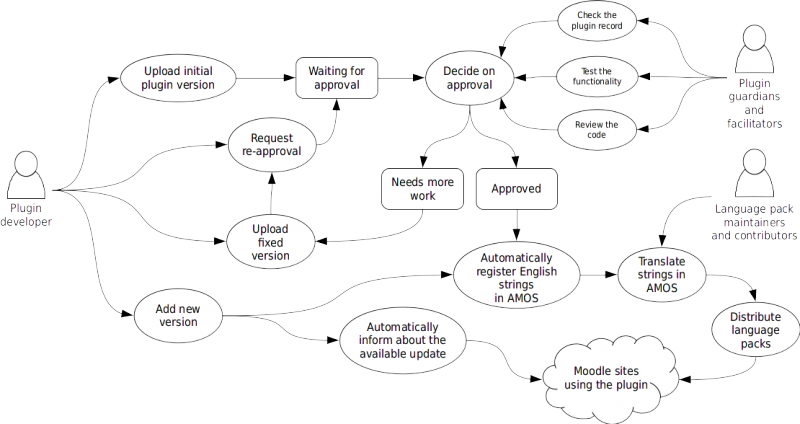
\includegraphics[scale=0.7]{images/plugin-contribution-workflow.png}
  \caption[Flux d'acception d'un module d'extension Moodle]{Flux d'acception d'un module d'extension Moodle, \href{https://docs.moodle.org/dev/Plugin_contribution}{\mbox{https://docs.moodle.org/dev/Plugin\_contribution}}}
\end{figure}

Pour ajouter des fonctionnalités à l'activité questionnaires, il y a trois types de module d'extensions à considérer: un rapport de questionnaire, un type de question et un comportement de question.

\subsection{Module d'extension rapport de questionnaire (\textit{Quiz report})}

Un rapport de questionnaire sert principalement à corriger les réponses des étudiants.
On peut aussi se servir de ce type de module d'extension pour afficher les réponses et les notes des étudiants pour un questionnaire sous forme de rapport.
On peut aussi s'en servir afin de modifier les champs disponibles dans la configuration de base d'un questionnaire.

Lors de l'analyse initiale du projet; il était prévu de se servir uniquement de ce type de module d'extension, car nous voulons uniquement modifier l'interface de correction.
Par contre, comme nous voulons ajouter une liste de mots clés à une question et que ce type de module d'extension permet de modifier seulement le questionnaire, un seul module d'extension de ce type ne sera pas suffisante.

\subsection{Module d'extension type de question (\textit{Question type})}

Chaque question est définie par un type de question (voir la liste à la section~1.1 de ce document).
Un nouveau type de question ajoute donc plus de choix à l'enseignant désirant créer un questionnaire.
Chaque type de question possède des champs personnalisés et change l'apparence de la question pour l'étudiant et l'enseignant.

On ne voulait pas modifier le module d'extension \og Type de question Composition \fg{} car les nouvelles fonctionnalités ne seront pas utiles pour tous les types de texte: un texte d'opinion pour un cours de philosophie, par exemple, n'aura aucune utilité d'une liste de mots-clés et de comparaison de textes.
La possibilité de créer un module d'extension qui ajoute un nouveau type de question qui étend les fonctionnalités du \og Type de question Composition \fg{} par héritage a été analysé, mais ce n'est pas possible avec Moodle.
Seule alternative restante: se baser sur le \og Type de question Composition \fg{} pour créer un tout nouveau module d'extension.
Ce nouveau module d'extension utilise les mêmes fonctionnalités que le \og Type de question Composition \fg{} en enlevant quelques fonctionnalités (remise de pièce jointe et écriture dans un WYSIWIG) et en ajoutant quelques autres (mots-clés et réponse de l'enseignant).

\subsection{Module d'extension comportement de question (\textit{Question behaviour})}

Un comportement de question permet de:
\begin{enumerate}
  \item Ajouter du code à la suite de la question, par exemple un bouton \og Vérifier \fg{} ou une zone de texte commentaire;
  
  \item Modifier la méthode de correction, par exemple une correction manuelle, une correction automatique instantanée quand l'étudiant répond ou une correction automatique lorsque le test est terminé;
  
  \item Modifier l'affichage des questions, par exemple afficher une question supplémentaire si l'étudiant a plusieurs fautes ou donner des indices à l'étudiant occasionnant une perte de points.
\end{enumerate}

Comme nous désirons une correction manuelle, nous pouvons utiliser le comportement \og ManualGraded \fg{}.
De plus, comme il est possible de contrôler directement l'apparence de la réponse et de la question avec le module d'extension \og Question type \fg{}, il n'est pas nécessaire de créer un module d'extension \og Comportement de question \fg{} pour modifier l'apparence de la question.

\section{Choix des modules d'extensions à créer}

Un module d'extension type de question est obligatoire dans ce projet afin d'ajouter les champs mots-clés et réponse de l'enseignant.
Nous n'avons pas besoin des fonctionnalités qu'offre le module d'extension comportement de question.
Il reste à déterminer s'il faut utiliser un module d'extension rapport de questionnaire ou non.

En analysant le code du module d'extension de correction manuelle fournie de base avec Moodle (quiz\_grading) on découvre qu'elle fournit l'interface de correction, mais que la réponse de chaque étudiant est gérée par le type de question dans un affichage en lecture seulement.
Les fonctionnalités prévues peuvent donc se trouver autant dans le type de question que dans un rapport de questionnaire, la complexité du code est la même pour les deux cas.
Puisqu'il doit y avoir obligatoirement un module d'extension type de question et qu'une nouveau module d'extension rapport de questionnaire est facultative, il a été décidé de faire un seul module d'extension.
Le fait d'avoir un seul module d'extension facilite grandement l'installation pour d'autres administrateurs Moodle.